\section{KYC process}

\begin{figure}[h!]
  \begin{sequencediagram}
    \newinst{wallet}{\shortstack{Customer \\
      \\ 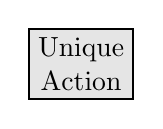
\begin{tikzpicture}
        \node [fill=gray!20,draw=black,thick,align=center] { Unique \\ Action};
      \end{tikzpicture}
    }}
    \newinst[2]{exchange}{\shortstack{Taler (exchange) \\
       \\ \begin{tikzpicture}[shape aspect=.5]
        \tikzset{every node/.style={cylinder,shape border rotate=90, draw,fill=gray!25}}
        \node at (1.5,0) {\shortstack{{{\tiny Database}}}};
       \end{tikzpicture}
    }}
    \newinst[2]{kyc}{\shortstack{KYC provider \\
       \\ \begin{tikzpicture}[shape aspect=.5]
        \tikzset{every node/.style={cylinder,shape border rotate=90, draw,fill=gray!25}}
        \node at (1.5,0) {\shortstack{{{\tiny Database}}}};
       \end{tikzpicture}
    }}

    \postlevel
    \mess[0]{wallet}{{Initial action}}{exchange}
    \begin{callself}{exchange}{Establish KYC requirement}{}
    \end{callself}
    \mess[0]{exchange}{Request new KYC process}{kyc}
    \mess[0]{kyc}{{Process identifier (PI)}}{exchange}
    \mess[0]{exchange}{{KYC required (PI)}}{wallet}
    \mess[0]{wallet}{{KYC start (PI)}}{kyc}
    \mess[0]{kyc}{{Request identity documentation}}{wallet}
    \mess[0]{wallet}{{Upload identity documentation}}{kyc}
    \begin{callself}{kyc}{Validate documentation}{}
    \end{callself}
    \mess[0]{kyc}{{Share documentation (PI)}}{exchange}
    \mess[0]{kyc}{{Confirm completion}}{wallet}
    \mess[0]{wallet}{{Retry action}}{exchange}
\end{sequencediagram}
  \caption{Deposit interactions between customer, Taler exchange (payment
    service provider) and external KYC provider.  The process can be
    triggered by various {\em actions} described in Chapter~\ref{chap:triggers}.}
  \label{fig:proc:kyc}
\end{figure}
